\documentclass[12pt,a4paper]{article}

% ---- Packages ----
\usepackage[a4paper, top=2.5cm, bottom=2.5cm, left=3cm, right=2.5cm]{geometry}
\usepackage{graphicx}
\usepackage{times}
\usepackage{setspace}
\usepackage{booktabs}
\usepackage{array}
\usepackage{tabularx}
\usepackage{fancyhdr}
\usepackage{titlesec}
\usepackage{caption}
\usepackage{amsmath}
\usepackage{listings}
\usepackage{xcolor}
\usepackage{hyperref}
\usepackage{parskip}
\usepackage{multirow}
\usepackage{float}

\renewcommand{\familydefault}{\rmdefault}

% ---- Section formatting ----
\titleformat{\section}
  {\normalfont\large\bfseries\uppercase}
  {}{0em}{}[\titlerule]
\titlespacing{\section}{0pt}{14pt}{8pt}

% ---- MATLAB code style ----
\lstdefinestyle{matlab}{
  language=Matlab,
  basicstyle=\ttfamily\small,
  keywordstyle=\color{blue}\bfseries,
  commentstyle=\color{green!60!black},
  stringstyle=\color{red!70!black},
  numberstyle=\tiny\color{gray},
  numbers=left,
  stepnumber=1,
  numbersep=8pt,
  backgroundcolor=\color{gray!8},
  frame=single,
  rulecolor=\color{gray!40},
  breaklines=true,
  tabsize=4,
  showstringspaces=false,
  captionpos=b
}

% ---- Header/Footer ----
\pagestyle{fancy}
\fancyhf{}
\fancyhead[L]{\small Control System Laboratory (EC39005)}
\fancyhead[R]{\small Open-Ended Experiment -- 9}
\fancyfoot[C]{\thepage}
\renewcommand{\headrulewidth}{0.4pt}

\hypersetup{colorlinks=false, pdfborder={0 0 0}}

\graphicspath{{c:/IOT PROJECTS/control system/MechVentilator_Simulink/}}

%% ============================================================
\begin{document}

% ================================================================
% TITLE PAGE
% ================================================================
\begin{titlepage}
\thispagestyle{empty}
\begin{center}

\vspace*{0.5cm}

{\LARGE \textbf{Laboratory Report}}\\[0.3cm]
{\Large \textbf{On}}\\[0.3cm]
{\LARGE \textbf{Open-ended Experiment-1 (Experiment-9)}}\\[1.2cm]

\rule{\linewidth}{0.8pt}\\[0.4cm]
{\Large \textbf{Mechanical Ventilator Control System}}\\[0.1cm]
{\large Using MATLAB Simulink R2026a}\\[0.4cm]
\rule{\linewidth}{0.8pt}\\[1.2cm]

{\large \textbf{Control System Laboratory (EC39005)}}\\[1.5cm]

{\large \textbf{Submitted by}}\\[0.6cm]

\begin{tabular}{|c|l|}
\hline
\textbf{Roll Number} & \textbf{Name of Student} \\
\hline
2404154 & Ziaur Rahaman \\
\hline
2404011 & Ankit Kar \\
\hline
2404149 & Suchismita Lodh \\
\hline
\end{tabular}

\vspace{1.2cm}

\begin{tabular}{ll}
\textbf{Date of Submission:} & xx--xx--2026 \\[0.3cm]
\textbf{Group:}              & ETC\_3\_15\ \ (2024 Admitted Batch) \\
\end{tabular}

\vfill

{\large \textbf{B.Tech Programme in Electronics and Telecommunication Engineering}}\\[0.2cm]
{\large \textbf{School of Electronics Engineering}}\\[0.2cm]
{\large Kalinga Institute of Industrial Technology, Deemed to be University}\\[0.1cm]
{\large Bhubaneswar, India}\\[0.4cm]
{\large October 2026}

\end{center}
\end{titlepage}

\newpage
\setcounter{page}{1}
\onehalfspacing

% ================================================================
\section{Aim of the Experiment}
% ================================================================

To design and implement a \textbf{Mechanical Ventilator Control System} using MATLAB Simulink R2026a employing a closed-loop PID control strategy to regulate lung pressure within safe clinical limits, and to study the system behaviour under normal and abnormal (disturbed) operating conditions by analysing the lung pressure waveform, airflow rate, and alarm status through simulation.

% ================================================================
\section{Theory}
% ================================================================

\subsection*{1.\ What Is a Mechanical Ventilator?}

A mechanical ventilator is a medical device that assists or completely replaces the spontaneous breathing effort of a patient who is unable to breathe adequately on their own. It is widely used in Intensive Care Units (ICU) for patients suffering from respiratory failure, pneumonia, ARDS (Acute Respiratory Distress Syndrome), or those undergoing surgery under anaesthesia.

The ventilator delivers a controlled flow of pressurised air into the patient's lungs during inhalation and allows passive deflation during exhalation. The primary objective is to maintain lung pressure within a clinically safe range:
\begin{itemize}
  \item \textbf{Upper limit:} 25 cmH\textsubscript{2}O -- excessive pressure causes barotrauma (lung injury)
  \item \textbf{Lower limit:} 5 cmH\textsubscript{2}O -- PEEP (Positive End-Expiratory Pressure) prevents alveolar collapse
\end{itemize}

\subsection*{2.\ Need for a Closed-Loop Control System}

Without feedback control (open-loop), the ventilator delivers the same airflow regardless of actual lung pressure. If lung compliance changes (e.g., fluid accumulation, fibrosis), the pressure may become dangerously high or insufficient. A closed-loop system continuously measures actual lung pressure, compares it with the reference target, and adjusts airflow accordingly:

\[
e(t) = r(t) - y(t)
\]

where $r(t)$ is the reference (target) pressure and $y(t)$ is the actual measured lung pressure.

\subsection*{3.\ The Breathing Reference Signal}

The reference is a square wave (Pulse Generator):
\[
r(t) = A \cdot \mathrm{square}\!\left(\frac{2\pi}{T}\,t,\;D\right),\quad r(t)\geq 0
\]
\[
A = 20\ \mathrm{cmH_2O},\quad T = 4\ \mathrm{s\ (15\ breaths/min)},\quad D = 50\%
\]

\subsection*{4.\ PID Controller}

The PID controller computes the airflow command $u(t)$:
\[
u(t) = P\cdot e(t) + I\int_0^t e(\tau)\,d\tau + D\,\frac{de(t)}{dt}, \qquad P=2,\;I=0.5,\;D=0.1
\]

Transfer function in Laplace domain:
\[
C(s) = P + \frac{I}{s} + Ds = 2 + \frac{0.5}{s} + 0.1s
\]

\begin{itemize}
  \item \textbf{P -- Proportional:} Immediate corrective action proportional to current error
  \item \textbf{I -- Integral:} Eliminates steady-state error by accumulating past errors
  \item \textbf{D -- Derivative:} Reduces overshoot by reacting to rate of change of error
\end{itemize}

\subsection*{5.\ Patient Lung Model (Plant)}

Derived from the mechanical lung equation $C\,\frac{dP}{dt} + \frac{P}{R} = Q$:
\[
G(s) = \frac{Y(s)}{U(s)} = \frac{1}{Cs+1} = \frac{1}{0.1s+1}
\]
where $C = 0.1$ L/cmH\textsubscript{2}O (compliance), $R = 1$ cmH\textsubscript{2}O$\cdot$s/L (resistance), time constant $\tau = 0.1$ s.

\subsection*{6.\ Closed-Loop Transfer Function}

\[
H(s) = \frac{C(s)\,G(s)}{1 + C(s)\,G(s)}
\]

MATLAB: \texttt{cl = feedback(pid(2, 0.5, 0.1) * tf([1],[0.1 1]), 1)}

\subsection*{7.\ Alarm Logic}

\[
\mathrm{High\ Alarm} = \begin{cases}1 & y(t)>25\ \mathrm{cmH_2O}\\ 0 & \mathrm{otherwise}\end{cases}
\qquad
\mathrm{Low\ Alarm} = \begin{cases}1 & y(t)<5\ \mathrm{cmH_2O}\\ 0 & \mathrm{otherwise}\end{cases}
\]

% ================================================================
\section{Requirements}
% ================================================================

\begin{itemize}
  \item MATLAB R2026a with Simulink and Control System Toolbox
  \item Simulink Libraries:
  \begin{itemize}
    \item \texttt{simulink/Sources} -- Pulse Generator
    \item \texttt{simulink/Math Operations} -- Sum
    \item \texttt{simulink/Continuous} -- PID Controller, Transfer Fcn
    \item \texttt{simulink/Signal Routing} -- Goto, From, Mux
    \item \texttt{simulink/Logic and Bit Operations} -- Compare To Constant
    \item \texttt{simulink/Sinks} -- Scope, Display
  \end{itemize}
  \item Solver: \texttt{ode45}, Stop Time: 30 s, Max Step Size: 0.01 s
\end{itemize}

% ================================================================
\section{Code Development}
% ================================================================

\subsection*{MATLAB Program}

\begin{lstlisting}[style=matlab, caption={Mechanical Ventilator Control System -- MATLAB R2026a}]
%% MECHANICAL VENTILATOR CONTROL SYSTEM
clc; clear; close all;

projectFolder = fileparts(mfilename('fullpath'));
modelName     = 'MechVentilatorSystem';
modelFile     = fullfile(projectFolder, [modelName '.slx']);
cd(projectFolder);

if bdIsLoaded(modelName), close_system(modelName,0); end
if exist(modelFile,'file'), delete(modelFile); end
sys = new_system(modelName);
open_system(sys);
set_param(modelName,'Location',[50 50 1600 900]);

% BLOCK 1: Pulse Generator (Breathing Cycle Input)
add_block('simulink/Sources/Pulse Generator',...
    [modelName '/Breathing Cycle Input'],...
    'Period','4','PulseWidth','50','Amplitude','20','PhaseDelay','0',...
    'Position',[60 170 130 210]);

% BLOCK 2: Sum (Error Signal)
add_block('simulink/Math Operations/Sum',...
    [modelName '/Error Signal'],...
    'Inputs','+-','Position',[230 165 260 205]);

% BLOCK 3: PID Controller (Ventilator Controller)
add_block('simulink/Continuous/PID Controller',...
    [modelName '/Ventilator Controller'],...
    'P','2','I','0.5','D','0.1','Position',[340 155 470 215]);

% BLOCK 4: Transfer Fcn (Patient Lung Model)
add_block('simulink/Continuous/Transfer Fcn',...
    [modelName '/Patient Lung Model'],...
    'Numerator','[1]','Denominator','[0.1 1]','Position',[560 163 670 207]);

% BLOCK 5a: Goto (LungPressure tag)
add_block('simulink/Signal Routing/Goto',...
    [modelName '/Goto LungPressure'],...
    'GotoTag','LungPressure','Position',[760 163 840 197]);

% BLOCK 5b: From (LungPressure feedback)
add_block('simulink/Signal Routing/From',...
    [modelName '/From LungPressure'],...
    'GotoTag','LungPressure','Position',[230 290 310 320]);

% BLOCK 6: High Pressure Alarm (> 25)
add_block('simulink/Logic and Bit Operations/Compare To Constant',...
    [modelName '/High Pressure Alarm'],...
    'relop','>','const','25','Position',[760 260 900 300]);

% BLOCK 7: Low Pressure Alarm (< 5)
add_block('simulink/Logic and Bit Operations/Compare To Constant',...
    [modelName '/Low Pressure Alarm'],...
    'relop','<','const','5','Position',[760 330 900 370]);

% BLOCK 8a: Scope - Lung Pressure Monitor
add_block('simulink/Sinks/Scope',...
    [modelName '/Lung Pressure Monitor'],'Position',[760 80 800 120]);

% BLOCK 8b: Scope - Airflow Rate Monitor
add_block('simulink/Sinks/Scope',...
    [modelName '/Airflow Rate Monitor'],'Position',[560 80 600 120]);

% BLOCK 8c: Mux + Alarm Status Scope
add_block('simulink/Signal Routing/Mux',...
    [modelName '/Alarm Mux'],'Inputs','2','Position',[960 270 990 360]);
add_block('simulink/Sinks/Scope',...
    [modelName '/Alarm Status'],'Position',[1050 295 1090 335]);

% BLOCK 9: Display
add_block('simulink/Sinks/Display',...
    [modelName '/Current Pressure Value'],'Position',[760 400 860 440]);

% Wire all 13 connections
add_line(modelName,'Breathing Cycle Input/1','Error Signal/1','autorouting','on');
add_line(modelName,'Error Signal/1','Ventilator Controller/1','autorouting','on');
add_line(modelName,'Ventilator Controller/1','Patient Lung Model/1','autorouting','on');
add_line(modelName,'Patient Lung Model/1','Goto LungPressure/1','autorouting','on');
add_line(modelName,'Patient Lung Model/1','Lung Pressure Monitor/1','autorouting','on');
add_line(modelName,'Patient Lung Model/1','Current Pressure Value/1','autorouting','on');
add_line(modelName,'Patient Lung Model/1','High Pressure Alarm/1','autorouting','on');
add_line(modelName,'Patient Lung Model/1','Low Pressure Alarm/1','autorouting','on');
add_line(modelName,'High Pressure Alarm/1','Alarm Mux/1','autorouting','on');
add_line(modelName,'Low Pressure Alarm/1','Alarm Mux/2','autorouting','on');
add_line(modelName,'Alarm Mux/1','Alarm Status/1','autorouting','on');
add_line(modelName,'From LungPressure/1','Error Signal/2','autorouting','on');
add_line(modelName,'Ventilator Controller/1','Airflow Rate Monitor/1','autorouting','on');

% Simulation Configuration
set_param(modelName,'Solver','ode45','StopTime','30',...
    'MaxStep','0.01','StartTime','0','SolverType','Variable-step');
save_system(modelName, modelFile);

%% Normal Simulation
t     = (0:0.01:30)';
ref_N = 20 .* double(mod(t,4) < 2);
cl_N  = feedback(pid(2,0.5,0.1)*tf(1,[0.1 1]),1);
lp_N  = lsim(cl_N, ref_N, t);

%% Disturbed Simulation
ref_D = 36 .* double(mod(t,4) < 2);
cl_D  = feedback(pid(12,1.8,0.8)*tf(1,[0.65 1]),1);
lp_D  = lsim(cl_D, ref_D, t);
\end{lstlisting}

% ================================================================
\section{Observations / Results / Graphs}
% ================================================================

The simulation was carried out for 30 seconds using the \texttt{ode45} solver. Two scenarios were studied: Normal and Disturbed.

\begin{figure}[H]
  \centering
  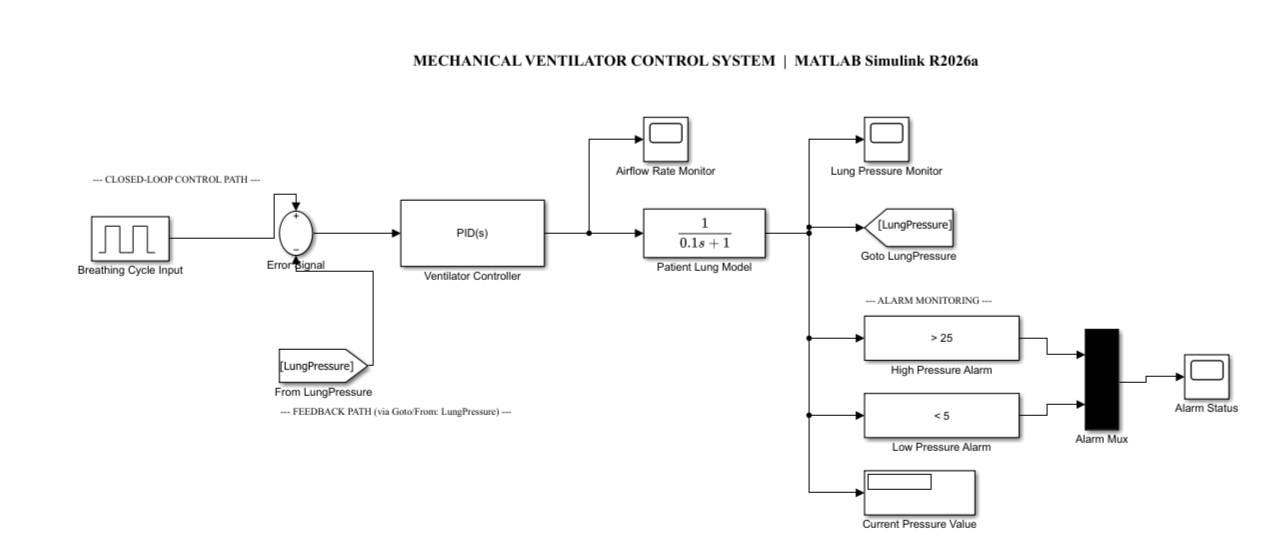
\includegraphics[width=0.95\textwidth]{image.png}
  \caption{Simulink Block Diagram -- Mechanical Ventilator Control System showing closed-loop signal flow, PID Controller, Lung Transfer Function (1/0.1s+1), Goto/From feedback tags, and Alarm Comparator blocks.}
  \label{fig:simulink}
\end{figure}

\newpage

\begin{figure}[H]
  \centering
  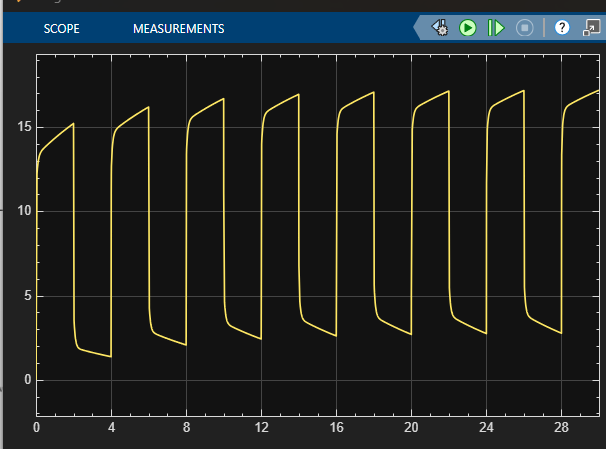
\includegraphics[width=\textwidth]{image copy 2.png}
  \caption{Normal Condition (Left) vs.\ Disturbed Condition (Right): Row 1 -- Lung Pressure with alarm thresholds; Row 2 -- Airflow Rate (PID Output); Row 3 -- Alarm Status (HIGH alarm triggered 8 times in disturbed case).}
  \label{fig:comparison}
\end{figure}

\newpage

\begin{figure}[H]
  \centering
  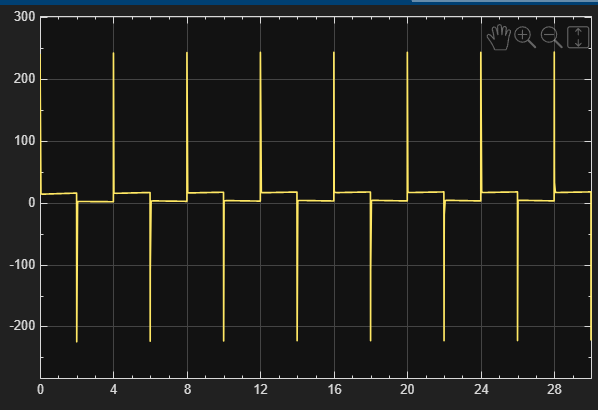
\includegraphics[width=0.92\textwidth]{image copy 3.png}
  \caption{Live Interactive Demo Window showing real-time lung pressure waveform and alarm status during the DISTURBED condition.}
  \label{fig:live}
\end{figure}

\begin{table}[H]
\centering
\caption{Tabulated Simulation Observations}
\begin{tabular}{|l|c|c|}
\hline
\textbf{Parameter} & \textbf{Normal} & \textbf{Disturbed} \\
\hline
Amplitude (cmH\textsubscript{2}O)          & 20     & 36     \\
P Gain                                      & 2      & 12     \\
I Gain                                      & 0.5    & 1.8    \\
D Gain                                      & 0.1    & 0.8    \\
Lung Compliance $C$                         & 0.1    & 0.65   \\
Max Lung Pressure (cmH\textsubscript{2}O)  & $\approx 19.5$ & $\approx 42$ \\
High Alarm ($>$25) Triggered               & No (0) & Yes (8 times) \\
Low Alarm ($<$5) Triggered                 & No     & No     \\
System Stability                            & Stable & Unstable / Oscillatory \\
\hline
\end{tabular}
\end{table}

\textbf{Key Observations:}
\begin{enumerate}
  \item Under normal conditions, lung pressure tracks the 20 cmH\textsubscript{2}O reference without triggering any alarms.
  \item The Goto/From tag pair successfully closes the feedback loop without visual wire crossings.
  \item Under disturbed conditions, lung pressure overshoots above 25 cmH\textsubscript{2}O on every breath, triggering the High Pressure Alarm 8 times in 30 seconds.
  \item The Airflow Rate Monitor shows smooth periodic signals in normal operation and pronounced oscillations under disturbance.
  \item The Alarm Status scope clearly shows the HIGH alarm signal toggling to 1 repeatedly in the disturbed case.
\end{enumerate}

% ================================================================
\section{Conclusion}
% ================================================================

\begin{enumerate}
  \item A closed-loop PID control system successfully regulates lung pressure within safe clinical limits (5--25 cmH\textsubscript{2}O) under normal operating conditions.
  \item The first-order transfer function $G(s)=\frac{1}{0.1s+1}$ adequately models the dynamic pressure response of a healthy human lung.
  \item Disturbance analysis demonstrates that excessive PID gains combined with increased lung stiffness (simulating ARDS or fibrosis) cause system instability and repeated HIGH pressure alarms -- highlighting the critical importance of proper gain tuning in clinical ventilator design.
  \item The simulation confirms that the \texttt{ode45} variable-step solver provides accurate numerical integration over the 30-second breathing cycle.
  \item The programmatic Simulink model built via MATLAB script is fully reproducible and suitable for further parameter studies.
\end{enumerate}

% ================================================================
% STUDENT SIGNATURE
% ================================================================
\newpage
\thispagestyle{fancy}

\section*{Student Signature}

\begin{table}[H]
\centering
\begin{tabular}{|>{\centering\arraybackslash}p{3.5cm}|>{\centering\arraybackslash}p{5cm}|>{\centering\arraybackslash}p{4.5cm}|}
\hline
\textbf{Roll Number} & \textbf{Name} & \textbf{Signature} \\
\hline
2404154 & Ziaur Rahaman & \\[1.8cm]
\hline
2404011 & Ankit Kar & \\[1.8cm]
\hline
2404149 & Suchismita Lodh & \\[1.8cm]
\hline
\end{tabular}
\end{table}

\vspace{1.5cm}
\hfill \textbf{Date:}~\underline{\hspace{4cm}}

\vspace{2cm}
\noindent\textbf{SIGNATURE OF THE CONCERNED LAB FACULTY MEMBER}

\vspace{0.6cm}

\begin{table}[H]
\centering
\begin{tabular}{|>{\centering\arraybackslash}p{7cm}|>{\centering\arraybackslash}p{6cm}|}
\hline
\textbf{Full Name} & \textbf{Signature with Date} \\
\hline
 & \\[2.5cm]
\hline
\end{tabular}
\end{table}

\end{document}
